\documentclass[10pt,a4paper]{article}
\usepackage[margin=24mm]{geometry}
\usepackage[T1]{fontenc}
\usepackage{lmodern,amsmath,amssymb,bm,graphicx,booktabs,microtype}
\usepackage{caption,float,placeins}
\usepackage[colorlinks=true,linkcolor=blue,citecolor=blue,urlcolor=blue]{hyperref}
\setlength{\emergencystretch}{2em}
\numberwithin{equation}{section}
\graphicspath{{figures/}}
\newcommand{\OPD}{\mathrm{OPD}}
\newcommand{\dd}{\,\mathrm{d}}
\newcommand{\NominalTable}{%
\begin{table}[htbp]
\centering
\caption{Nominal inputs for the reported calculations.}\label{tab:parameters}
\begin{tabular}{ll}\toprule
Quantity & Value\\\midrule
Substrate radius $R$ & $12.7$ mm\\
Substrate thickness $L$ & $5.0$ mm\\
Beam radius $w_0$ & $3.81$ mm ($0.3R$)\\
Full-plane absorbed power $P_{\rm abs}$ & $0.110$ W\\
Thermal conductivity $k$ & $1.38$ W\,m$^{-1}$\,K$^{-1}$\\
Density $\rho$ & $2203$ kg\,m$^{-3}$\\
Specific heat $c_p$ & $772$ J\,kg$^{-1}$\,K$^{-1}$\\
Ambient temperature $T_\infty$ & $300$ K\\
Convection coefficient $h_{\rm conv}$ & $10$ W\,m$^{-2}$\,K$^{-1}$\\
Emissivity $\epsilon$ & $0.85$\\
Linearized total loss $h_{\rm eff}$ & $15.2054$ W\,m$^{-2}$\,K$^{-1}$\\
Thermo-optic coefficient $\gamma_T$ & $9.6\times10^{-6}$ K$^{-1}$\\
Reference wavelength; refractive indices & $1064$ nm; $n_i=1$, $n_s=1.44963$\\
Entrance-pupil radius $a$ & $0.9R$\\\bottomrule
\end{tabular}
\par\smallskip\begin{minipage}{.96\linewidth}\footnotesize $\gamma_T$ is a retained nominal value tabulated at $643.8$ nm, not a wavelength-specific measurement at $1064$ nm. The intercepted disk power is obtained by integrating the prescribed flux on the finite face.\end{minipage}
\end{table}}

\newcommand{\SteadyFieldTable}{%
\begin{table}[htbp]
\centering
\caption{Steady temperature rises and sampled OPD-PV.}\label{tab:steadyfields}
\begin{tabular}{lrrrr}\toprule
$\theta$ & Front center (K) & Midplane center (K) & Rear center (K) & OPD-PV (nm)\\\midrule
$0^\circ$ & 11.921 & 7.656 & 6.716 & 166.503\\
$30^\circ$ & 11.336 & 7.537 & 6.656 & 168.771\\
$60^\circ$ & 9.303 & 6.959 & 6.314 & 154.105\\\bottomrule
\end{tabular}
\par\smallskip\begin{minipage}{.96\linewidth}\footnotesize OPD-PV uses the saved $201\times201$ physical transmitted-pupil grid. Continuous numerical extrema are reported separately in Supplement 1; FEM comparisons use their own discrete common domain.\end{minipage}
\end{table}}

\newcommand{\TransientRefinementTable}{%
\begin{table}[htbp]
\centering
\caption{Largest transient FEM refinement changes across temperature and OPD metrics (percent).}\label{tab:refinement}
\begin{tabular}{lrrrr}\toprule
$\theta$ & Transverse & Axial & Time & Joint\\\midrule
$0^\circ$ & 0.104616 & 0.029993 & 0.025763 & 0.125259\\
$30^\circ$ & 0.099671 & 0.029973 & 0.025837 & 0.118577\\
$60^\circ$ & 0.088451 & 0.029925 & 0.026017 & 0.105834\\
Target & $0.5$ & $0.5$ & $0.1$ & $0.5$\\\bottomrule
\end{tabular}
\par\smallskip\begin{minipage}{.96\linewidth}\footnotesize Maxima include the positive observation times from $0.0025$ to $75$ s. The $0.001$ s frame is recorded separately as a diagnostic; the exact zero initial condition and all-step physical checks remain independent requirements.\end{minipage}
\end{table}}

\newcommand{\ValidationTable}{%
\begin{table}[htbp]
\centering
\caption{Optical differences between FEM and the semi-analytical calculation (percent).}\label{tab:comparison}
\begin{tabular}{lrrr}\toprule
$\theta$ & Steady $E_V$ & Transient $E_V$ & Transient $E_{W,\infty}$\\\midrule
$0^\circ$ & 0.004220 & 0.071263 & 0.090254\\
$30^\circ$ & 0.000523 & 0.054394 & 0.085118\\
$60^\circ$ & 0.005440 & 0.046821 & 0.082570\\\bottomrule
\end{tabular}
\par\smallskip\begin{minipage}{.96\linewidth}\footnotesize Steady values use the finest FEM mesh. Transient values are maxima over sampled times from $2.5$ ms to $75$ s and use the FEM candidate examined by the separate refinements. All denominators are the semi-analytical PV on the common pupil. Supplement 1 retains full temperature and optical statistics, including $1$ ms diagnostics.\end{minipage}
\end{table}}

\title{A Fourier--Bessel semi-analytical model for steady and transient thermo-optic response of finite cylindrical optics under oblique Gaussian surface heating}
\author{Zhongwei Yang, Jing Wen, Wei Li, Tingrui Li, Bohui Chen, and Liang Yang}
\date{Working draft for author review: 27 October 2026}
% Author-approved structure: six sections, 27 October 2026.
% Physical authority: PHYSICAL_MODEL.md in the author-supplied handoff ZIP.
% Saved evidence: outputs/experiment_audit/20261017T121521368371Z_f107298c;
% its 281 snapshot-file hashes were checked before this revision.
% TODO(science): comparison runs retain transient_truncation_established=false,
% although separate selection checks pass. Preserve both states; do not claim
% complete scientific acceptance or silently promote the suite's not_run state.
% The historical runs used a dirty bac2146 tree and recorded source hashes;
% they are not fresh runs of the current manuscript commit.
\begin{document}
\maketitle
\begin{abstract}
% para:abstract-p01
Oblique irradiation of a coated cylindrical optic changes both the surface-heating footprint and the paths along which transmitted light samples the temperature field.
We develop a Fourier--Bessel semi-analytical model for the three-dimensional steady and transient temperature rise under a prescribed Gaussian surface heat flux and Robin heat-loss conditions.
The transient solution combines the steady axial response with homogeneous axial diffusion modes and is evaluated directly at specified times.
Integration along fixed refracted reference rays gives the transmitted substrate thermo-refractive optical-path difference (OPD).
For nominal fused-silica cases at external angles of $0^\circ$, $30^\circ$, and $60^\circ$, recorded comparisons with independently assembled three-dimensional finite-element solutions give maximum OPD peak-to-valley differences of $0.00544\%$ in steady state and $0.0713\%$ over the sampled step-response times from $1$ ms to $75$ s, normalized by the semi-analytical values.
The $1$ ms comparison is diagnostic; the FEM refinement targets apply from $2.5$ ms onward.
Azimuthal analysis distinguishes temperature-field shares from the OPD contributions obtained by integrating each thermal order along the refracted paths, which need not retain the same angular structure in the entrance pupil.
\end{abstract}

\section{Introduction}
% para:intro-p01
Absorption in a laser-irradiated coating produces a nonuniform temperature field in the optical substrate.
The resulting refractive-index variation changes the optical path of the transmitted light.
Dichroic mirrors used in wavelength beam combining provide a representative application: studies have examined their temperature rise and the influence of thermal deformation on beam quality \cite{li2024,li2025}.
For oblique Gaussian incidence, the surface-heating footprint is elliptical, and the refracted rays traverse different transverse positions through the substrate.
Predicting the transmitted thermo-refractive OPD therefore requires the spatial temperature distribution along those paths, rather than a single temperature value.

% para:intro-p02
Analytical and semi-analytical descriptions of laser-induced thermal effects provide a basis for this calculation.
Peng et al.\ \cite{peng2001} used Green's functions to calculate temperature distributions and thermal deformations of finite cylindrical mirror substrates under Gaussian absorption.
Kim et al.\ \cite{kim2017} used Bessel functions to describe steady heating and thermal lensing in cylindrical optics.
Vinet \cite{vinet2009} developed non-axisymmetric Fourier--Bessel representations for steady mirror temperatures and treated axisymmetric transient responses and thermal lensing.
For oblique illumination, Reitzle et al.\ \cite{reitzle2021} derived a semi-analytical transient temperature solution for a laterally infinite, layered scattering and absorbing slab.
These formulations establish eigenfunction and transform methods for different thermal geometries, source distributions, and optical settings.

% para:intro-p03
We consider a finite cylindrical substrate heated by coating absorption from a single obliquely incident Gaussian beam and evaluate the thermo-refractive OPD of its transmitted branch.
The calculation couples a non-axisymmetric surface heat flux, heat exchange at the circular sidewall and both end faces, and an optical integral along fixed Snell-refracted reference rays.
A Fourier--Bessel representation also separates the azimuthal temperature contributions during diffusion.
Each contribution can be integrated along the same refracted rays, allowing its optical effect to be examined alongside its share of the temperature field.
Because the rays shift transversely with depth, the thermal order does not, in general, identify an angular Fourier order of the final entrance-pupil OPD.

% para:intro-p04
The principal contribution is a semi-analytical formulation for steady and transient temperature fields and the resulting transmitted substrate thermo-refractive OPD in this configuration.
The two thermal solutions share the transverse eigenfunctions and heat-flux projections; homogeneous axial diffusion modes describe the transient response at requested times without thermal time stepping.
We examine finite modal resolution and compare the calculated fields with independently assembled three-dimensional FEM solutions for the nominal cases.
The results then relate the incidence-angle dependence, transient diffusion, and azimuthal temperature structure to the OPD sampled along the refracted paths.
Section 2 defines the physical model and optical quantity, Section 3 develops the formulation, Section 4 presents numerical checks and FEM comparisons, and Section 5 discusses the thermal and optical results.

\section{Physical Model and Thermo-Optic OPD}
\subsection{Geometry and Oblique Gaussian Heating}
% para:model-p01
A cylindrical substrate of radius $R$ and thickness $L$ occupies $0\leq r\leq R$, $0\leq\phi<2\pi$, and $0\leq z\leq L$.
The coordinate origin is at the center of the coated front face, $z=0$; the rear face is at $z=L$.
We use $x=r\cos\phi$ and $y=r\sin\phi$.
A single collimated Gaussian beam is centered on the front face and propagates in the $y$--$z$ plane at an external angle $\theta$ to the $+z$ normal.
Its $1/e^2$ intensity radius in a plane normal to propagation is $w_0$.
The coating's absorbed power supplies a prescribed surface heat flux, while the transmitted part of the same beam enters the substrate.
The model heat flux is
\begin{equation}
 q_s(x,y)=\frac{2P_{\rm abs}\cos\theta}{\pi w_0^2}
 \exp\!\left[-\frac{2(x^2+y^2\cos^2\theta)}{w_0^2}\right].
 \label{eq:source}
\end{equation}
The footprint widths are $w_0$ along $x$ and $w_0/\cos\theta$ along $y$.
The normalization is $\int_{\mathbb R^2}q_s\dd A=P_{\rm abs}$, so $P_{\rm abs}$ is a prescribed full-plane heat-source power, not the incident laser power.
The power intercepted by the finite substrate is $P_{\mathcal D}=\int_{r\leq R}q_s\dd A$; the flux is not renormalized after clipping to the disk.
The angle comparisons hold $P_{\rm abs}$ fixed and do not calculate the coating's angle-, wavelength-, or polarization-dependent absorptance.
A prescribed normalized history $g(t)$ gives the applied flux $g(t)q_s$.

\begin{figure}[htbp]
% TODO(figure, author): move the origin to the front-face center and replace
% the historical centered-coordinate face labels by z=0 and z=L.
\centering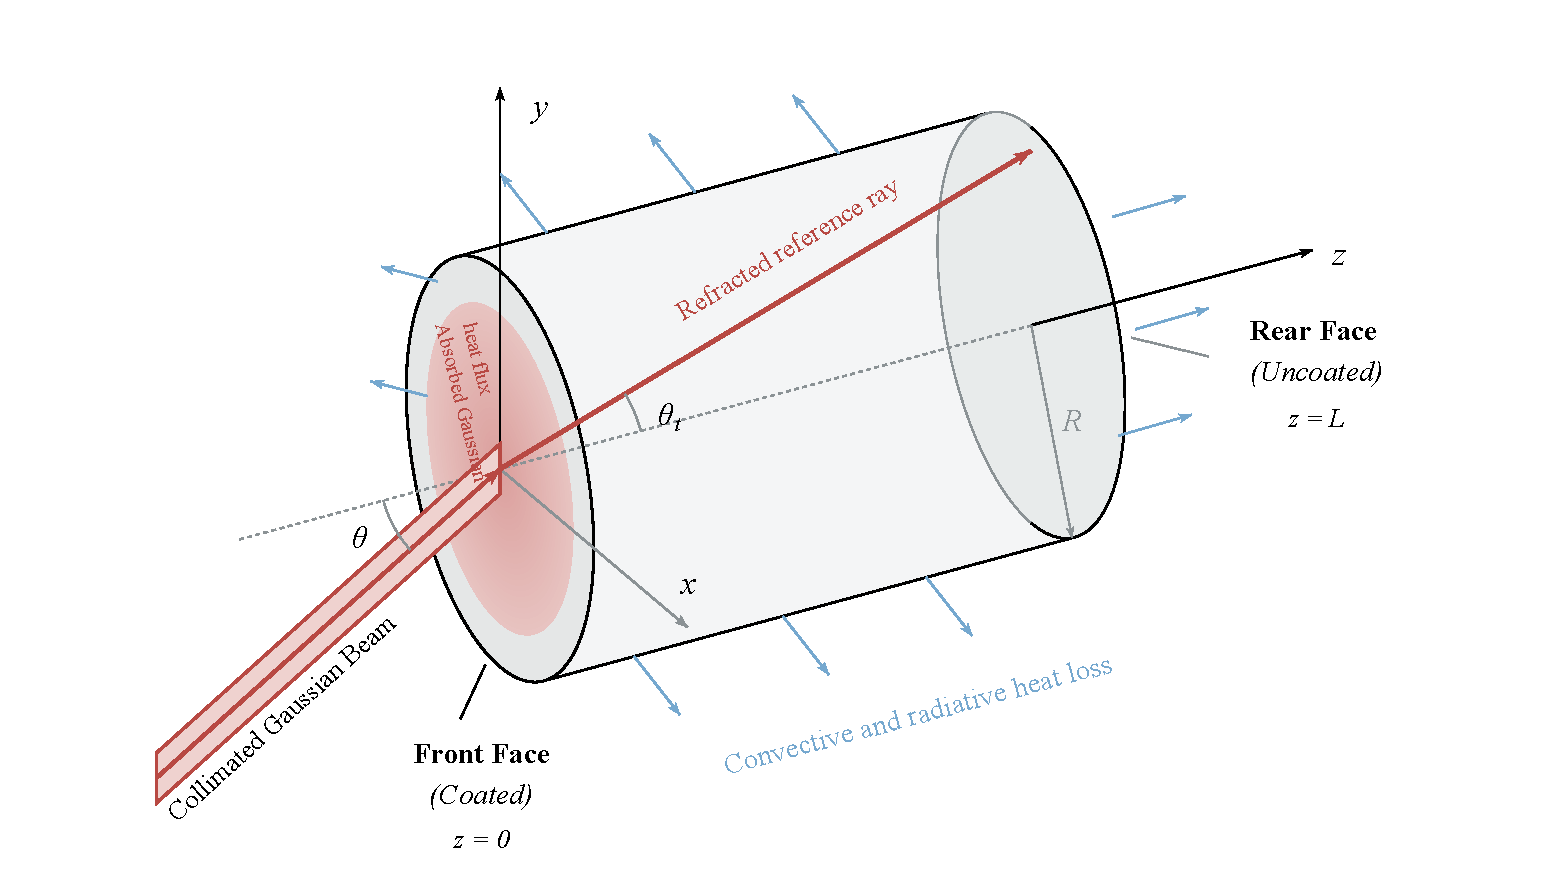
\includegraphics[width=.95\linewidth]{fig_physical_model_schematic_final.pdf}
\caption{Finite cylindrical substrate under oblique Gaussian coating-surface heating and environmental heat loss. The retained illustration awaits the author\textquotesingle s coordinate revision: its centered origin and $z=\pm L/2$ labels are superseded by the front-face origin and $z=0,L$ used throughout the text. The transmitted reference ray is defined by Eq.~\eqref{eq:ray}.}
\label{fig:geometry}
\end{figure}

\subsection{Heat-Transfer Model}
% para:model-p02
Let $\Theta=T-T_\infty$ be the temperature rise above ambient.
With thermal conductivity $k$, density $\rho$, and specific heat $c_p$, the substrate satisfies
\begin{equation}
 \rho c_p\frac{\partial\Theta}{\partial t}=k\nabla^2\Theta,
 \qquad \Theta(r,\phi,z,0)=0.
 \label{eq:heat}
\end{equation}
There is no volumetric heat source in this model.
The surface conditions are
\begin{align}
 h_f\Theta-k\partial_z\Theta&=g(t)q_s, &&z=0,\label{eq:front}\\
 h_b\Theta+k\partial_z\Theta&=0, &&z=L,\label{eq:rear}\\
 h_s\Theta+k\partial_r\Theta&=0, &&r=R.\label{eq:side}
\end{align}
Thus heating and environmental loss act simultaneously on the front face.
These signs follow from the outward normal on each surface.
In the nominal calculation all three heat-transfer coefficients equal
\begin{equation}
 h_{\rm eff}=h_{\rm conv}+4\epsilon\sigma T_\infty^3,
 \label{eq:heff}
\end{equation}
where $\sigma$ is the Stefan--Boltzmann constant and the second term is the linearization of radiative exchange about ambient.
Under constant loading, the steady field satisfies $\nabla^2\Theta_{\rm ss}=0$ with the corresponding stationary surface conditions.

\subsection{Assumptions and Nominal Inputs}
% para:model-p03
The substrate is homogeneous and isotropic, and its material properties are treated as constants.
The coating thickness is unresolved: coating absorption supplies the prescribed front-face heat flux, while bulk absorption is omitted.
Uniform Robin coefficients describe environmental heat loss.
The model does not resolve a mount, spatially varying contact conductance, or nonlinear radiative exchange.
The beam position, width, angle, and spatial profile are fixed during each thermal history.
We demonstrate an ideal step, with $g(0)=0$ and $g(t)=1$ for $t>0$.
Other histories can enter the modal convolution derived in Sec.~\ref{sec:transient}, but the reported three-dimensional comparisons concern this step-loading case.

% para:model-p04
Table~\ref{tab:parameters} specifies a nominal fused-silica example.
The geometry, beam size, absorbed power, convection coefficient, and emissivity define the numerical case rather than measured specifications of a particular mounted component.
The conductivity, density, and specific heat follow the cited quartz-glass data~\cite{heraeus}; $c_p$ is held at the tabulated mean over $0$--$100\,{}^\circ$C.
The optical coefficient $\gamma_T=\mathrm dn/\mathrm dT=9.6\times10^{-6}\,\mathrm{K}^{-1}$ is retained as a nominal input tabulated at $643.8$ nm, rather than a measured coefficient at the $1064$ nm reference wavelength.
The reference refractive index is $n_s=1.44963$.
For fixed thermal parameters and reference rays, the calculated OPD scales linearly with the adopted $\gamma_T$.
\NominalTable

\subsection{Thermo-Optic OPD along Refracted Rays}
% para:model-p05
The transmitted reference ray obeys $n_i\sin\theta=n_s\sin\theta_t$, where $n_i$ and $n_s$ are the external and unheated substrate refractive indices.
A ray entering at $(x_0,y_0,0)$ follows
\begin{equation}
 x(z)=x_0,\quad y(z)=y_0+z\tan\theta_t,\quad \dd s=\frac{\dd z}{\cos\theta_t}.
 \label{eq:ray}
\end{equation}
Its first-order thermo-optic OPD relative to the unheated substrate is
\begin{equation}
 W(x_0,y_0,t)=\frac{\gamma_T}{\cos\theta_t}
 \int_0^L\Theta\!\left(x_0,y_0+z\tan\theta_t,z,t\right)\dd z.
 \label{eq:opd}
\end{equation}
Entrance coordinates label the field.
The physical transmitted pupil is the intersection of $x_0^2+y_0^2\leq a^2$, with $a=0.9R$, and $x_0^2+(y_0+L\tan\theta_t)^2\leq R^2$.
Convexity then keeps the full ray inside the cylinder.
The valid pupil therefore depends on angle; FEM comparisons additionally restrict it to the common mesh domain.
The peak-to-valley value is $V=\max W-\min W$ over the specified pupil.
The raw OPD retains piston relative to the unheated reference ray, while field-difference norms use a piston-removed field.
Equation~\eqref{eq:opd} includes only the first-order substrate refractive-index contribution on the fixed reference path; thermoelastic displacement, stress-optic changes, coating phase, and thermal ray bending are outside this optical model.

\section{Fourier--Bessel Semi-Analytical Formulation}
\subsection{Azimuthal Decomposition}
% para:method-p01
We express the spatial source in angular Fourier components,
\begin{equation}
 q_s(r,\phi)=q_0(r)+\sum_{m=1}^{\infty}q_m(r)\cos(m\phi),
 \label{eq:fourier}
\end{equation}
where $q_0=(2\pi)^{-1}\int_0^{2\pi}q_s\dd\phi$ and $q_m=\pi^{-1}\int_0^{2\pi}q_s\cos(m\phi)\dd\phi$ for $m>0$.
For the centered source in Eq.~\eqref{eq:source}, reflection symmetry removes sine terms, and $\pi$-periodicity removes odd cosine orders.
The retained set is therefore $m=0,2,4,\ldots,M$.
Normal incidence leaves only $m=0$.
At oblique incidence, the higher even orders encode the elliptical footprint without changing the circular substrate geometry.

\subsection{Fourier--Bessel Projection}
% para:method-p02
The radial functions are $J_m(\lambda_{mn}r)$, where the positive roots satisfy the sidewall condition,
\begin{equation}
 k\lambda_{mn}J_m'(\lambda_{mn}R)+h_sJ_m(\lambda_{mn}R)=0.
 \label{eq:radial}
\end{equation}
Define $N_{mn}=\int_0^R J_m^2(\lambda_{mn}r)r\dd r$ and $A_m=2\pi$ for $m=0$, $A_m=\pi$ otherwise.
The surface-flux coefficients are
\begin{equation}
 C_{mn}=\frac{\displaystyle\int_0^R\!\int_0^{2\pi}
 q_s(r,\phi)J_m(\lambda_{mn}r)\cos(m\phi)r\dd\phi\dd r}{A_mN_{mn}}.
 \label{eq:projection}
\end{equation}
These coefficients have units of heat flux.
The radial norm can be evaluated as
\begin{equation}
 N_{mn}=\frac{R^2}{2}\left[J_m^2(\lambda_{mn}R)
       -J_{m-1}(\lambda_{mn}R)J_{m+1}(\lambda_{mn}R)\right].
\end{equation}
With finite truncation, the reconstructed source is $q_{MN}=\sum_{m,n}C_{mn}J_m\cos(m\phi)$.
Root accuracy, source quadrature, and truncation are checked separately; satisfying the retained modal boundary condition alone does not establish convergence to the prescribed Gaussian flux.

\subsection{Steady-State Solution}
% para:method-p03
For each transverse mode, the steady axial amplitude satisfies $Z_{mn}''-\lambda_{mn}^2Z_{mn}=0$ and the two plane-face conditions.
Setting $\lambda=\lambda_{mn}$ gives
\begin{equation}
 Z_{mn}^{\rm ss}(z)=C_{mn}\frac{\cosh[\lambda(L-z)]+\frac{h_b}{k\lambda}\sinh[\lambda(L-z)]}
 {(k\lambda+\frac{h_fh_b}{k\lambda})\sinh(\lambda L)+(h_f+h_b)\cosh(\lambda L)}.
 \label{eq:steadyaxial}
\end{equation}
The assembled steady temperature is
\begin{equation}
 \Theta_{\rm ss}(r,\phi,z)=\sum_{m,n}J_m(\lambda_{mn}r)\cos(m\phi)Z_{mn}^{\rm ss}(z).
 \label{eq:steady}
\end{equation}
The implementation evaluates an equivalent decaying-exponential form of Eq.~\eqref{eq:steadyaxial} to avoid large hyperbolic intermediate values.
Temperature and analytical radial and axial derivatives follow from the same expansion.
The optical integral in Eq.~\eqref{eq:opd} is evaluated at the displaced ray coordinates, rather than replacing the ray by a fixed transverse position.

\subsection{Transient Solution}\label{sec:transient}
% para:method-p04
The transverse basis and source coefficients remain unchanged in the transient problem.
We introduce homogeneous axial Robin eigenfunctions
\begin{equation}
 X_j(z)=\cos(\beta_jz)+\frac{h_f}{k\beta_j}\sin(\beta_jz),\qquad
 \mathcal N_j=\int_0^L X_j^2(z)\dd z,
 \label{eq:axialmodes}
\end{equation}
normalized by $X_j(0)=1$.
Their positive roots obey
\begin{equation}
 \left(\frac{h_fh_b}{k^2}-\beta_j^2\right)\sin(\beta_jL)
  +\frac{h_f+h_b}{k}\beta_j\cos(\beta_jL)=0.
 \label{eq:axialroots}
\end{equation}
Writing $\alpha=k/(\rho c_p)$, the decay rate of a complete thermal mode is
\begin{equation}
 d_{mnj}=\alpha(\lambda_{mn}^2+\beta_j^2).
 \label{eq:rate}
\end{equation}
The indices $n$ and $j$ describe independent radial and axial resolutions.
In particular, one decay rate per radial mode does not represent the full finite-thickness transient.

% para:method-p05
For the surface forcing, projection onto the homogeneous axial functions yields the causal amplitude
\begin{equation}
 Z_{mn}(z,t)=\frac{C_{mn}}{\rho c_p}
 \sum_{j=0}^{\infty}\frac{X_j(z)}{\mathcal N_j}
 \int_0^t e^{-d_{mnj}(t-s)}g(s)\dd s.
 \label{eq:convolution}
\end{equation}
For a unit step and $t>0$, the exact steady amplitude is the sum of the stationary modal terms.
The response can consequently be written
\begin{align}
 Z_{mn}(z,t)&=Z_{mn}^{\rm ss}(z)
       -\sum_{j=0}^{\infty}B_{mnj}X_j(z)e^{-d_{mnj}t},\label{eq:completion}\\
 B_{mnj}&=\frac{C_{mn}}{k\mathcal N_j(\lambda_{mn}^2+\beta_j^2)}.\nonumber
\end{align}
The evaluated approximation retains the first $J$ decaying terms in Eq.~\eqref{eq:completion} and keeps $Z_{mn}^{\rm ss}$ in its exact modal form.
The rapidly decaying axial tail is thereby completed by the steady response.
At $t=0$ the specified zero initial field is returned exactly.
At positive times, $J$ is selected against enlarged references, including the earliest requested time; finite $J$ does not guarantee uniform accuracy as $t\to0^+$.

% para:method-p06
The resulting temperature has the same spatial sum as Eq.~\eqref{eq:steady}, with $Z_{mn}^{\rm ss}$ replaced by $Z_{mn}(z,t)$.
Each requested time is evaluated directly from the decay factors.
For the step response, $t\to\infty$ removes the decaying terms and recovers the same retained steady solution.
The decaying correction satisfies homogeneous Robin conditions, while the steady term carries the nonhomogeneous front-face load.
This separation preserves the boundary structure at every evaluated positive time and permits reuse of the steady projection, spatial evaluation, derivatives, and ray integration.


\subsection{OPD Evaluation and Thermal-Order Contributions}
% para:method-p07
The optical integral is evaluated by Gauss--Legendre quadrature along each valid refracted reference ray.
Let $\Theta_m(r,z,t)\cos(m\phi)$ denote the temperature component assembled from all retained radial and axial terms of thermal order $m$.
Its OPD contribution is
\[
 W_m(x_0,y_0,t)=\frac{\gamma_T}{\cos\theta_t}
 \int_0^L\Theta_m\bigl(r(z),z,t\bigr)\cos\bigl(m\phi(z)\bigr)\dd z,
 \qquad W=\sum_m W_m,
\]
where $r(z)$ and $\phi(z)$ are obtained from Eq.~\eqref{eq:ray}.
This sum follows from the linear optical integral on fixed paths.
The index $m$ labels the temperature contribution entering the integral; the functions $W_m$ are not assumed to be angular Fourier modes of the entrance pupil.
Their individual peak-to-valley amplitudes are diagnostic quantities and cannot be added to obtain the peak-to-valley value of $W$.

\section{Numerical Verification and FEM Comparison}
\subsection{Modal Resolution and Sampling}
% para:results-p01
The numerical examples use the geometry and material inputs in Table~\ref{tab:parameters} and external angles $0^\circ$, $30^\circ$, and $60^\circ$.
Steady resolution selection gives $M=6$, $N=8$, with a $400\times32$ source-projection grid and 16 ray-quadrature points.
The transient selection gives $M=10$, $N=20$, $J=256$, a $1200\times128$ projection grid, and 32 ray points.
Both selections compare temperature and OPD with enlarged finite references at a $0.1\%$ target.
The transient checks additionally resolve temperature gradients and diffusion-layer depths.
Their positive reference times are $0.001$, $0.0025$, $0.01$, $0.05$, $0.1$, $0.625$, $2.5$, $20$, $50$, and $75$ s.
Zero initial conditions and a separate long-time limit are checked independently.

% para:validation-p00
The steady finite reference uses $M=14$, $N=32$, a $2400\times256$ projection grid, and 64 ray points; the enlarged reference uses $M=16$, $N=40$, a $3200\times512$ grid, and 80 ray points.
The transient references use those transverse settings with $J=512$ and $768$, respectively.
These checks assess changes between finite numerical representations at the stated angles and samples, rather than an exact-solution error bound.
The exact zero initial condition is distinct from positive-time convergence of the truncated axial expansion.
\emph{Author-review note:} the individual modal-selection checks are available, but the combined truncation status of the transient cross-method runs remains unresolved; the differences below are reported at the recorded resolutions.
% TODO(science): the separate modal-selection checks pass, but the historical
% comparison summaries retain transient_truncation_established=false and the
% aggregate scientific status is not_run. Reconcile these records before
% describing the complete transient calculation as scientifically accepted.

\subsection{FEM Formulation and Refinement}

% para:validation-p01
The finite-element model uses the same prescribed Gaussian flux, geometry, material parameters, and Robin losses, with an independent nodal thermal representation.
It employs quadratic functions on a triangular transverse mesh and quadratic axial elements, with a consistent mass matrix for transient diffusion.
It does not use the Fourier--Bessel source coefficients to construct the applied load.
The steady checks vary the transverse mesh, axial mesh, and both together, giving maximum changes below $0.081\%$ at all three angles against a $0.1\%$ target.
Temperature and OPD are compared on common physical domains, excluding locations outside the inscribed finite-element boundary.
Figure~\ref{fig:steadyfem} displays the reconstructed distributions and signed field differences for $60^\circ$.
\begin{figure}[htbp]
\centering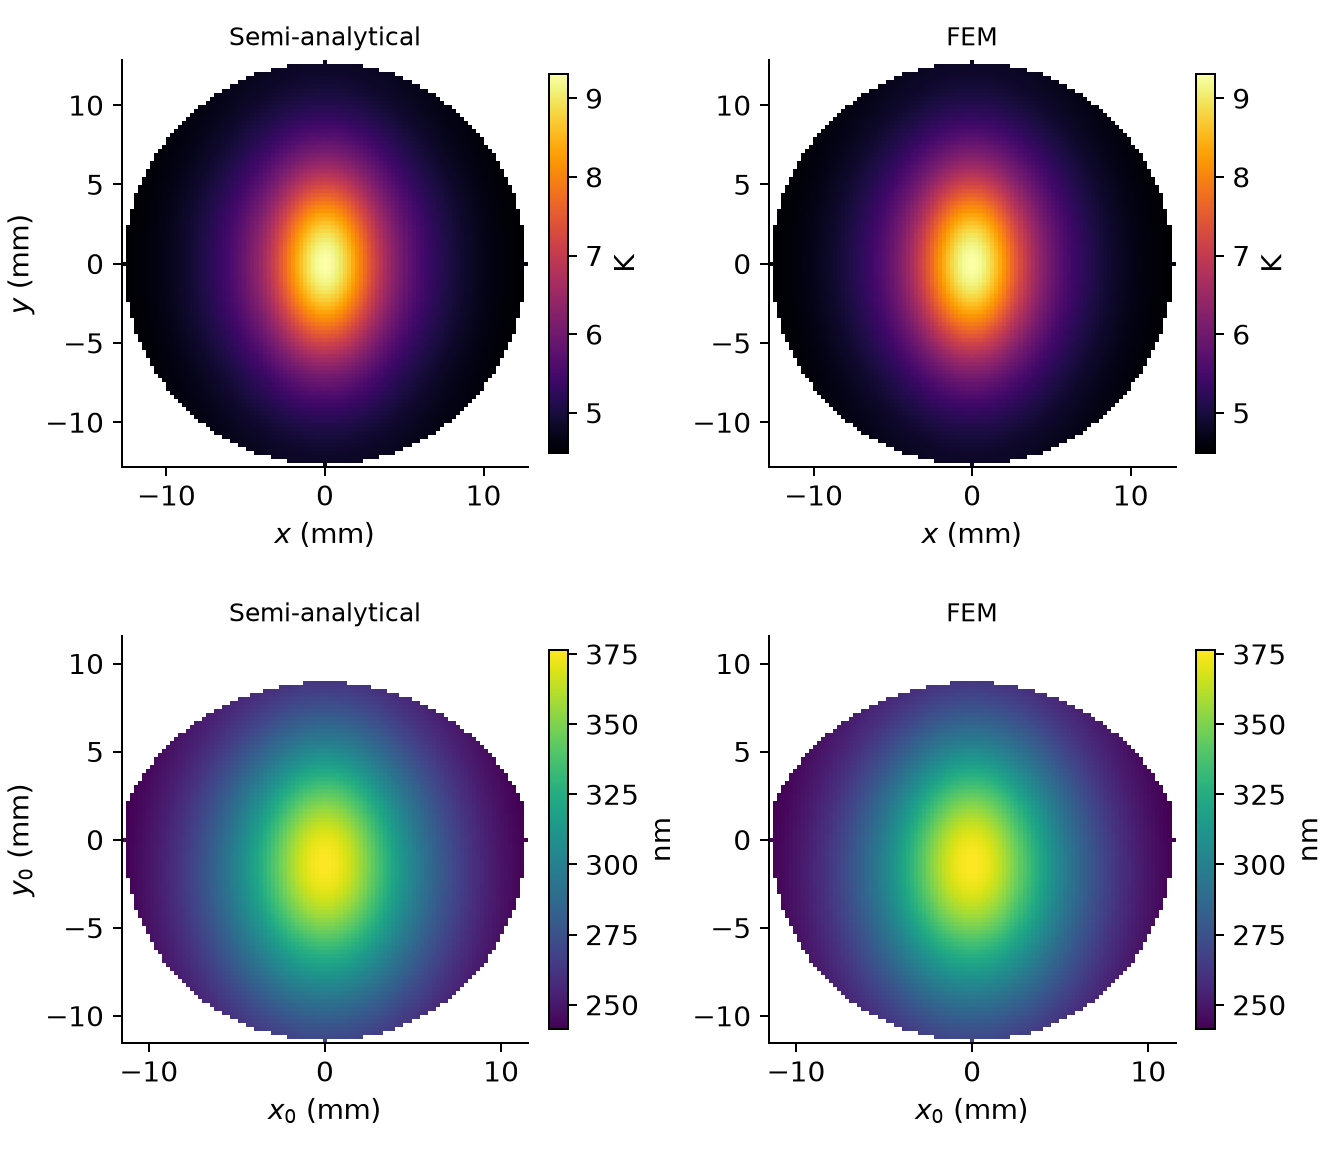
\includegraphics[width=\linewidth]{steady_fem_comparison.png}
\caption{Steady $60^\circ$ distribution comparison on the common domain: semianalytical field, finest finite-element field, and finite-element minus semianalytical difference. Top: front-plane temperature rise. Bottom: refracted-ray OPD, with piston removed from the difference. The two methods use independent thermal representations.}
\label{fig:steadyfem}
\end{figure}

% para:validation-p02
Transient finite-element calculations use BDF2 time integration with backward-Euler starts or restarts in the recorded time plan.
Spatial and temporal convergence are examined independently before a joint refinement.
The candidate and the transverse, axial, time, and joint references are evaluated at the same eleven observation times, including zero.
Table~\ref{tab:refinement} gives the maximum changes across the recorded temperature and OPD metrics.
The spatial and joint targets are $0.5\%$, while the time target is $0.1\%$.
The $1$ ms frame is retained as an early-time diagnostic and is excluded from these finite-element refinement gates; it remains part of the semianalytical truncation selection and of the reported cross-method comparisons.
Initial conditions, energy balance, weak-equation residuals, Robin-loss diagnostics, and applied-load quadrature are checked separately.
The refinement comparisons use a $201\times201$ Cartesian thermal grid and a $101\times101$ optical grid within their respective common masks.
\TransientRefinementTable

% para:validation-p02b
The steady meshes have $2113$ or $8321$ transverse degrees of freedom and $32$ or $64$ uniform quadratic axial elements, giving $137345$, $540865$, $272577$, and $1073409$ total degrees of freedom for the candidate, transverse, axial, and joint configurations.
For the transient problem, the corresponding transverse counts are unchanged.
Two-face axial grading gives $88$ elements ($177$ axial degrees of freedom) for the candidate and $174$ elements ($349$ axial degrees of freedom) for the axial reference.
Thus the transient candidate has $374001$ total degrees of freedom and the joint reference has $2904029$.
The ten successive observation intervals use $128$ steps each, except $0.1$--$0.625$ s, which uses $1024$, for $2176$ steps in total.
Time and joint references halve every interval step.
A backward-Euler step starts the calculation and restarts BDF2 when the step ratio exceeds $1.5$.
The Gaussian load uses quadrature order 10 and is checked against order 14; the resulting changes satisfy the $10^{-5}$ relative target.
Refracted-ray FEM integrals are split at crossed element boundaries and use three-point Gauss quadrature on each segment.
The tensor-product quadratic field is quartic along a straight segment, so this optical integration is exact for the represented field up to arithmetic error.

\subsection{Temperature and OPD Comparison}
% para:validation-p03
For cross-method temperature comparison, weighted $L^2$ differences are divided by the reference $L^2$ norm and maximum differences by the reference maximum magnitude.
At $t\geq0.625$ s each section uses its own denominator; at earlier positive times each norm uses its largest reference value across the three sections, avoiding division by the vanishing norm of an almost unheated rear plane.
For OPD, let $\widetilde W=W-\langle W\rangle$ on the common pupil.
The reported field and scalar metrics are
\begin{equation}
 E_{W,\infty}=\frac{\max|\widetilde W_{\rm FEM}-\widetilde W_{\rm SA}|}{V_{\rm SA}},\quad
 E_{W,2}=\frac{\operatorname{rms}(\widetilde W_{\rm FEM}-\widetilde W_{\rm SA})}{V_{\rm SA}},\quad
 E_V=\frac{|V_{\rm FEM}-V_{\rm SA}|}{V_{\rm SA}}.
 \label{eq:errors}
\end{equation}
The normalization by OPD-PV is distinct from a pointwise relative error and remains meaningful at locations where the piston-removed OPD crosses zero.

% para:validation-p04
Table~\ref{tab:comparison} reports the cross-method differences.
For the steady comparisons, the OPD-PV difference is at most $0.00544\%$ and the piston-removed maximum field difference is at most $0.0712\%$ of the reference PV.
For the transient comparisons over all recorded positive times, including $1$ ms, the corresponding maxima are $0.0713\%$ and $0.0958\%$.
The largest normalized transient temperature maximum difference is $0.137\%$.
These are differences at the recorded modal and FEM resolutions, rather than error bounds relative to an exact solution or a measured device wavefront.
Figure~\ref{fig:transientfem} additionally shows the spatial OPD differences at an early and a later time.
\ValidationTable
\begin{figure}[htbp]
\centering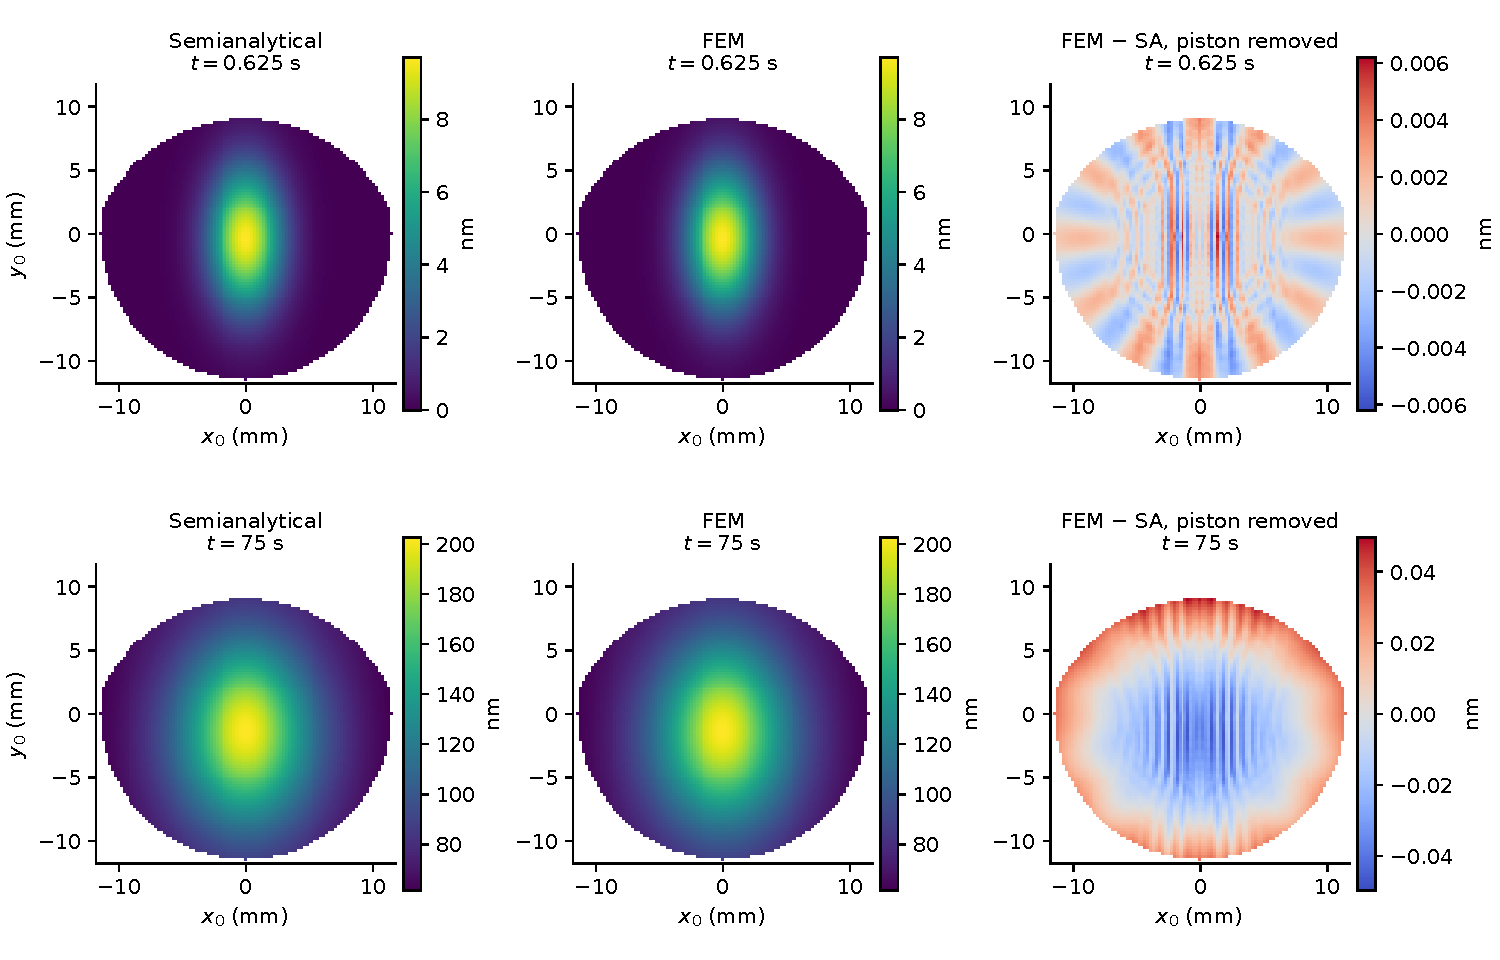
\includegraphics[width=\linewidth]{transient_fem_comparison.pdf}
\caption{Refracted-ray OPD at $60^\circ$ and $t=0.625$ s (top) and $75$ s (bottom): semianalytical field, refined-candidate FEM field, and their piston-removed difference. Each row uses a shared scale for the two optical fields.}
\label{fig:transientfem}
\end{figure}

\FloatBarrier
\section{Results and Discussion}
\subsection{Steady-State Temperature and OPD under Oblique Incidence}
% para:results-p02
Figure~\ref{fig:steadyfields} shows the $30^\circ$ steady temperature and OPD fields for the nominal inputs in Table~\ref{tab:parameters}.
The front, middle, and rear center temperature rises are $11.336$, $7.537$, and $6.656$ K, respectively.
The temperature distribution broadens through the thickness, while the OPD integrates the temperature along a ray whose transverse position changes with depth.
Table~\ref{tab:steadyfields} compares the three angles: the front-center temperature rise decreases from $11.921$ to $11.336$ to $9.303$ K, whereas OPD-PV takes the values $166.503$, $168.771$, and $154.105$ nm.
Thus the front-center temperature alone does not determine the ordering of OPD-PV in these three cases.
The source width and peak flux, the temperature distribution, the refracted path, and the valid pupil all enter the calculation as the angle changes.
The present angle comparison varies them together; it does not isolate their separate quantitative contributions to the observed OPD-PV trend.
\SteadyFieldTable
\begin{figure}[htbp]
\centering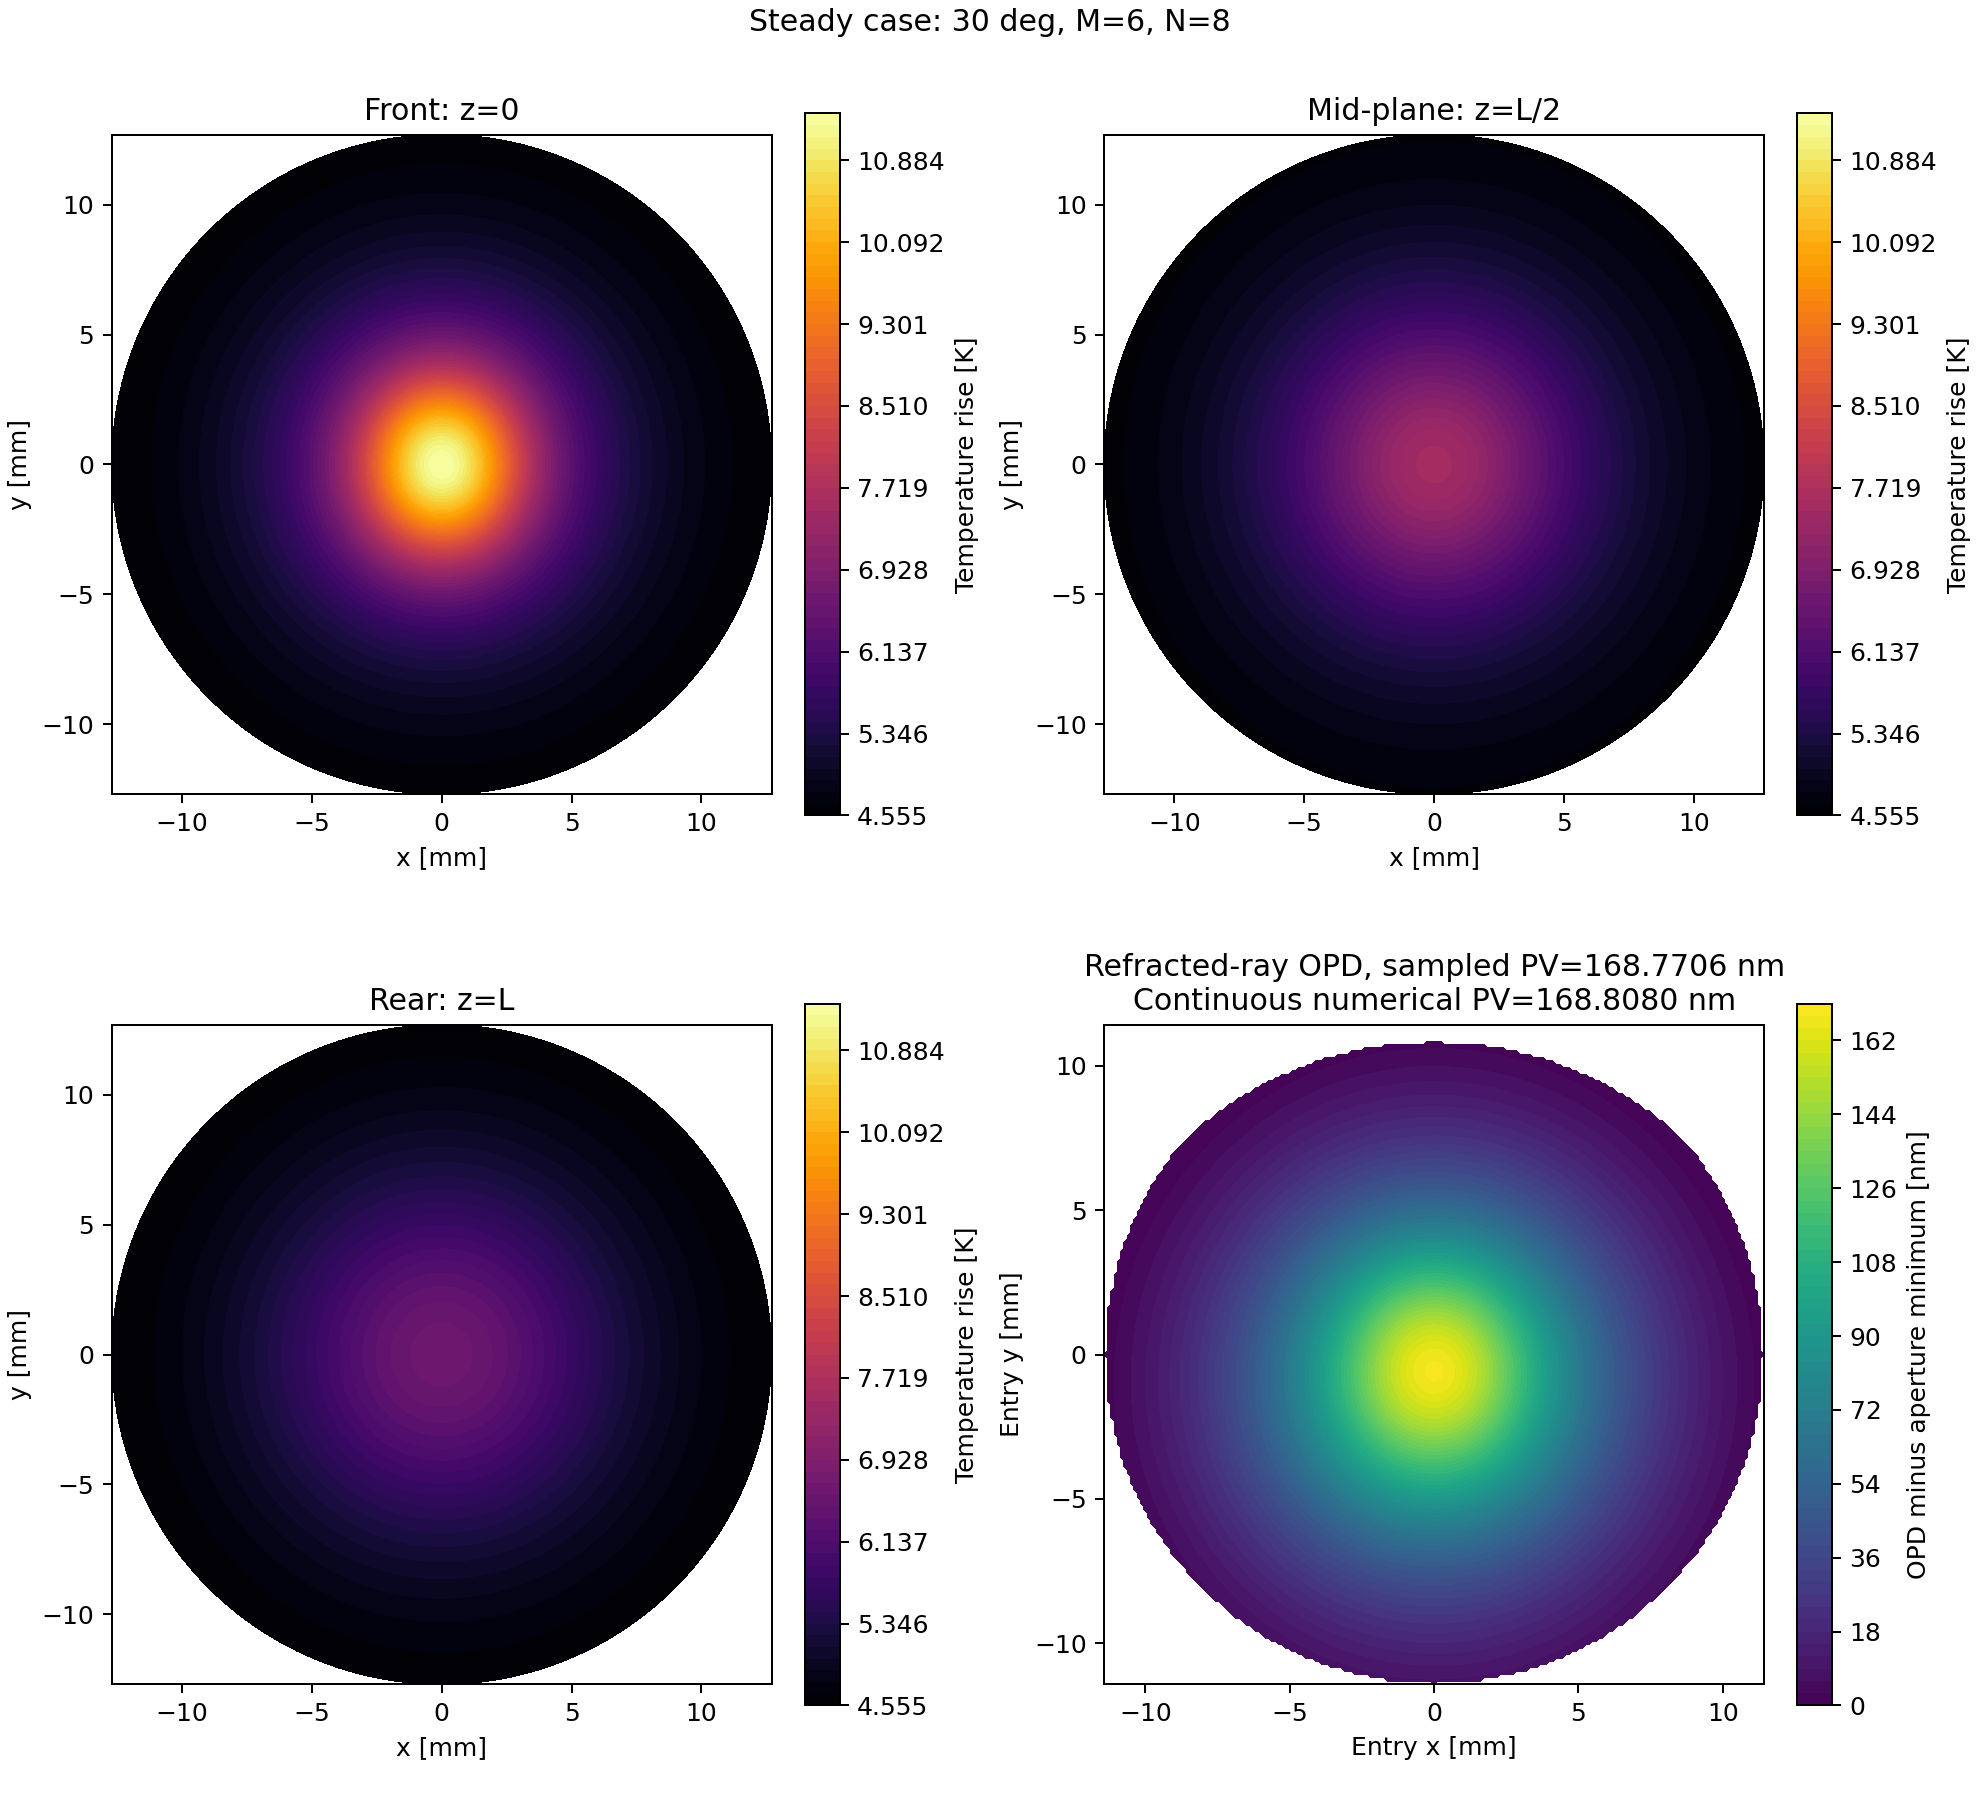
\includegraphics[width=.83\linewidth]{representative_steady.png}
\caption{Representative $30^\circ$ steady temperature rises on the front, middle, and rear planes, and transmitted thermo-optic OPD. OPD is shown relative to its pupil minimum for visualization. Coordinates on the optical panel are entrance coordinates.}
\label{fig:steadyfields}
\end{figure}

\subsection{Transient Evolution of Temperature and OPD}
% para:results-p03
Figure~\ref{fig:evolution} follows the temperature and OPD after step turn-on.
Heating is initially concentrated near the illuminated face, and diffusion subsequently extends the temperature rise through the substrate.
The front-center temperature samples a single position, whereas OPD accumulates temperature along the full refracted path; their amplitudes therefore describe different aspects of the evolving field.
At $0.625$ s, the continuous numerical OPD-PV values are $14.922$, $13.932$, and $9.700$ nm for $0^\circ$, $30^\circ$, and $60^\circ$, respectively.
At $75$ s, they are $156.347$, $156.966$, and $140.781$ nm.
The $75$ s frame is an intermediate response rather than the imposed steady endpoint.
A separate evaluation at approximately $2447$ s differs from the same-mode steady OPD-PV by at most $7.6\times10^{-5}\%$ across the three angles.
That limit uses the transient modal resolution for both solutions, so the comparison isolates the remaining temporal correction.
\begin{figure}[htbp]
\centering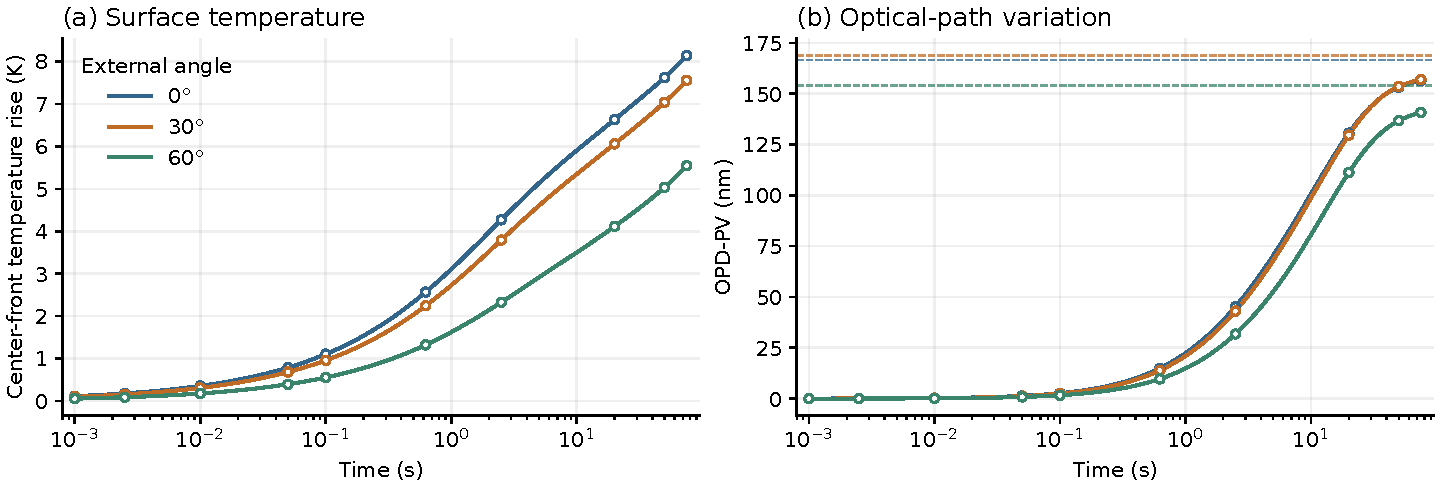
\includegraphics[width=.98\linewidth]{transient_evolution.pdf}
\caption{Time development under step loading: (a) center-front temperature rise and (b) pupil OPD-PV for the three incidence angles. Curves show sampled direct modal evaluations. Circles identify the finite-reference comparison times; dashed lines in (b) show the respective same-mode steady limits.}
\label{fig:evolution}
\end{figure}

\subsection{Azimuthal Thermal Modes and Their OPD Contributions}
% para:modes-p01
Obliquity first changes the source through its $y$-direction width and its angular Fourier content.
The circular sidewall and uniform loss coefficients preserve the independence of the azimuthal thermal orders, so each source order can be propagated through the substrate separately.
For a spatial temperature component $\Theta_m(r,z,t)\cos(m\phi)$, define its section-wise squared-$L^2$ share as
\begin{equation}
 S_m(z,t)=\frac{\displaystyle\int_0^{2\pi}\!\int_0^R
 |\Theta_m(r,z,t)\cos(m\phi)|^2r\dd r\dd\phi}
 {\displaystyle\sum_\ell\int_0^{2\pi}\!\int_0^R
 |\Theta_\ell(r,z,t)\cos(\ell\phi)|^2r\dd r\dd\phi}.
 \label{eq:share}
\end{equation}
Orthogonality makes these shares additive on the full circular section.
They describe temperature-field magnitude, not stored thermal energy, whose integral is linear in temperature.

% para:modes-p02
The saved modal results identify $m=2$ as the largest non-axisymmetric front-surface temperature contribution at the reported times for $30^\circ$ and $60^\circ$.
At $30^\circ$, its squared-$L^2$ share decreases from $0.513\%$ at $1$ ms to $0.0521\%$ at $75$ s.
At $60^\circ$, the corresponding values are $9.92\%$ and $1.34\%$, while the $m=4$ share decreases from $0.827\%$ to $0.0486\%$.
Figure~\ref{fig:modes} shows the $60^\circ$ thermal shares alongside the OPD amplitudes obtained from the same thermal orders.
The surface shares describe the relative temperature structure at one depth; they do not include the path integration used for OPD.

% para:modes-p03
For the optical contributions defined in Section 3, let $V_m=\max W_m-\min W_m$ on the sampled transmitted pupil.
At $60^\circ$, $V_2$ increases from $4.203$ nm at $0.625$ s to $28.752$ nm at $75$ s, while its front-surface temperature share decreases over that interval.
The corresponding sampled total OPD-PV values are $9.700$ and $140.778$ nm.
The decreasing thermal share and increasing $V_2$ are compatible because one is a relative squared temperature norm on a section and the other is an absolute optical amplitude after integration through the thickness.
Although the fields satisfy $W=\sum_mW_m$, their extrema occur at potentially different pupil positions, so the individual $V_m$ values are not additive fractions of the total OPD-PV.
\begin{figure}[htbp]
% Saved figure copied without alteration from:
% outputs/transient_case/20261016T200140235063Z_8f3a1290_p2_full_transient_fields_theta60_a1/figures/transient_modes.png
\centering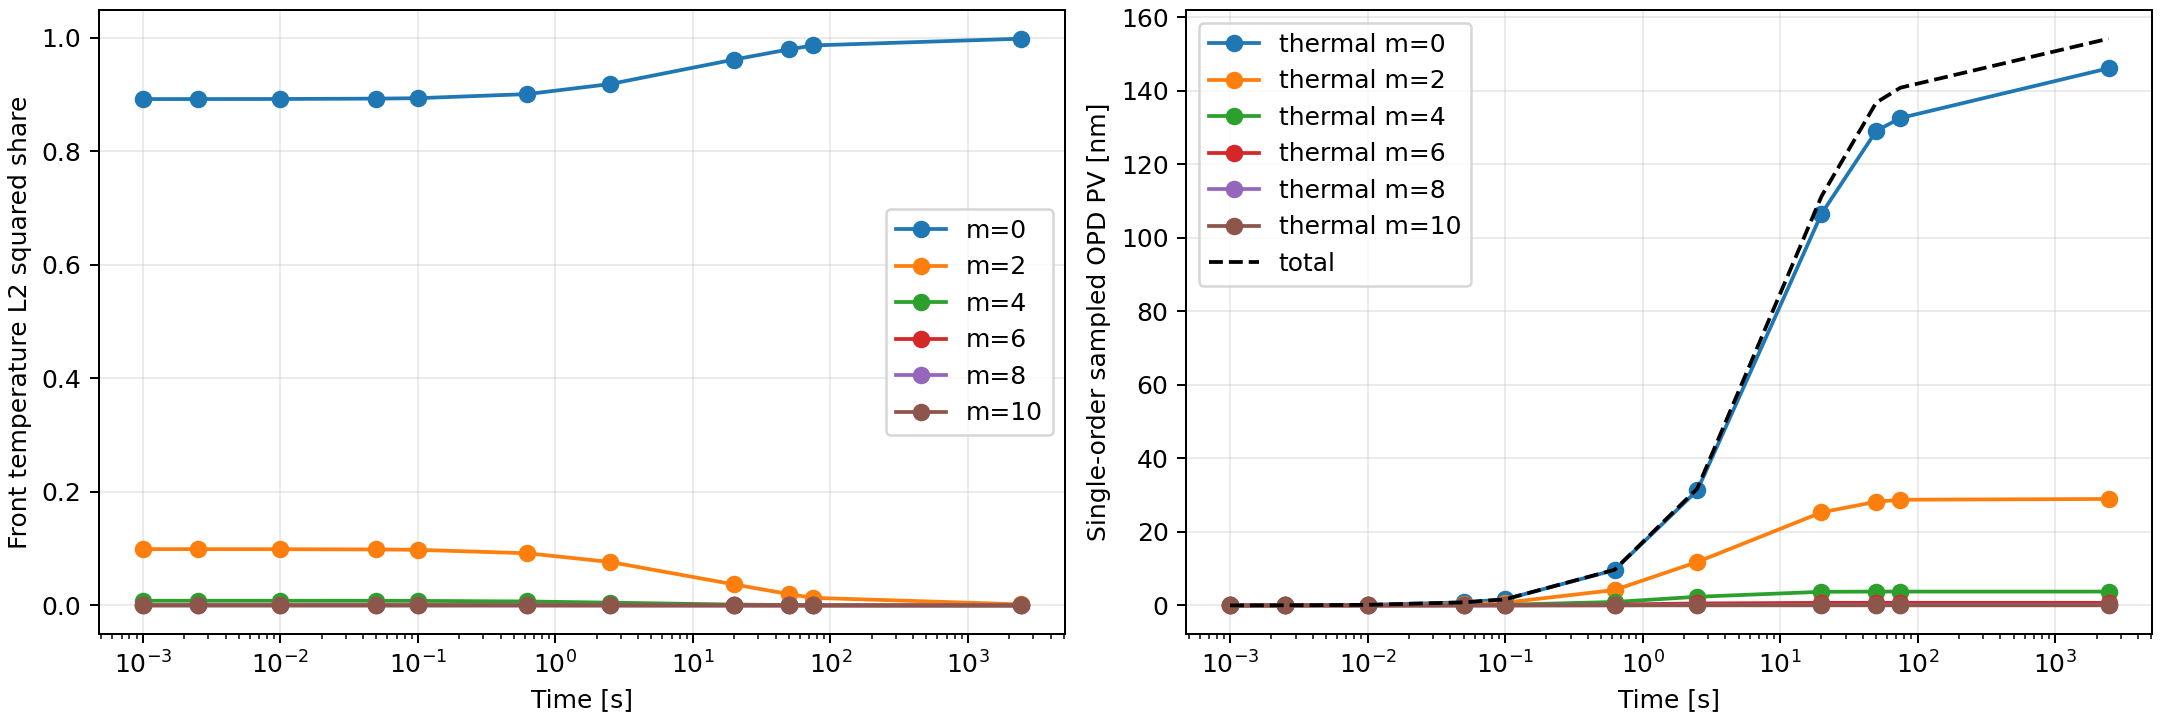
\includegraphics[width=\linewidth]{azimuthal_contributions_60deg.png}
\caption{Thermal-order contributions at $60^\circ$ under step loading. Left: front-surface squared-$L^2$ temperature shares. Right: individual sampled OPD-PV amplitudes $V_m$ obtained by integrating each thermal order along the refracted rays; the dashed curve is the PV of the summed field. Individual PV amplitudes are not additive. The last point is the separate long-time evaluation at approximately $2447$ s; preceding points extend to $75$ s. Thermal order labels do not denote angular Fourier modes of the entrance-pupil OPD.}
\label{fig:modes}
\end{figure}


% para:modes-p04
\begin{samepage}
The difference in spatial structure follows directly from the ray geometry.
For an axisymmetric temperature contribution, the radius sampled at depth $z$ is $r(z)=\sqrt{x_0^2+(y_0+z\tan\theta_t)^2}$.
At oblique incidence, entrance points with the same radius can therefore sample different temperatures along their paths, and the transmitted pupil itself is restricted by the exit condition.
Consequently, an axisymmetric $m=0$ temperature field need not produce an axisymmetric OPD about the entrance-face origin.
The modal decomposition separates the thermal origins of the OPD contributions; resolving angular orders of the final OPD would require a separate decomposition on a specified optical pupil.

\end{samepage}

\subsection{Scope and Limitations}
% para:scope-p01
The model applies to coating-dominated absorption in a homogeneous cylinder with approximately constant properties and linear surface losses.
A measured or calculated absorbed-power history can replace the ideal step through Eq.~\eqref{eq:convolution}.
Bulk absorption would require a distributed source term, and a thermally conducting mount would require an appropriate contact-boundary model.
Temperature-dependent properties and nonlinear radiation would couple the retained modes and change the linear response.
The nominal thermo-optic coefficient used here sets the OPD scale; device-specific predictions require a coefficient appropriate to the actual material and wavelength.

% para:scope-p02
The optical calculation concerns the first-order refractive-index contribution on the fixed transmitted reference ray.
Thermoelastic changes in surface position, stress-optic effects, and the coating's optical phase can contribute to the measured wavefront and should be included when those quantities are required.
The present three-angle comparisons assess the stated nominal thermal problem numerically.
They do not replace a temperature or wavefront measurement for a particular mounted component.
The recorded comparisons start at $1$ ms, which is retained as a diagnostic outside the FEM refinement gates; the gated FEM range starts at $2.5$ ms.
The exact initial condition and positive-time modal convergence remain separate requirements.

\section{Conclusion}
% para:conclusion-p01
We have developed a Fourier--Bessel semi-analytical formulation for a finite cylindrical substrate under single-beam oblique Gaussian surface heating.
The steady axial response and homogeneous axial diffusion modes share a transverse representation, allowing steady and transient temperature fields to be evaluated and integrated along fixed refracted reference rays.
For the nominal three-angle cases, recorded FEM comparisons give maximum steady and transient OPD-PV differences of $0.00544\%$ and $0.0713\%$, respectively, relative to the semi-analytical values and within the comparison settings of Section 4.
The transient maximum includes the diagnostic $1$ ms frame; the FEM refinement targets apply to the sampled times from $2.5$ ms to $75$ s.

% para:conclusion-p02
\begin{samepage}
The results distinguish local temperature changes, section-wise thermal structure, and the transmitted OPD obtained by sampling the full depth along refracted paths.
Across the three incidence angles, the front-center temperature and OPD-PV exhibit different trends.
The azimuthal analysis further shows why a temperature mode's relative surface share need not track its absolute OPD amplitude, and why a thermal order does not generally remain an angular Fourier order in the entrance pupil.
The formulation therefore provides both a calculation of the substrate thermo-refractive contribution and a means of examining how the spatial temperature field enters that optical quantity.

\end{samepage}

\FloatBarrier
% Reference metadata and claim locations rechecked 27 October 2026.
% Detailed reading scope and access debts: working/reading_ledger.md.
\begin{thebibliography}{99}
% VERIFIED 2026-10-27: publisher PDF and Crossref DOI record.
% https://api.crossref.org/works/10.1016/j.optcom.2023.130034
\bibitem{li2024}
D. Li, X. Niu, J. Xia, H. Jiao, X. Dun, J. Zhang, X. Cheng, and Z. Wang,
``Research on the core factors affecting the temperature rise of dichroic mirrors in wavelength beam combination system under high-power CW laser,''
\emph{Optics Communications} \textbf{552}, 130034 (2024).
\href{https://doi.org/10.1016/j.optcom.2023.130034}{doi:10.1016/j.optcom.2023.130034}.
% VERIFIED 2026-10-27: publisher metadata; full-text Sec.1, 2.1 and 3.4 read.
% https://link.springer.com/article/10.1007/s00340-021-07718-2
% Version-of-record year is 2022; the DOI contains 2021.
\bibitem{dobek2022}
K. Dobek,
``Thermal lensing: outside of the lasing medium,''
\emph{Applied Physics B} \textbf{128}, 18 (2022).
\href{https://doi.org/10.1007/s00340-021-07718-2}{doi:10.1007/s00340-021-07718-2}.
% VERIFIED 2026-10-27: local publisher full text and Crossref record.
% https://api.crossref.org/works/10.1051/jphys:0199000510120126700
% SUPPORT: pp.1272--1273, Eqs.12--21; pp.1279--1280, Eqs.29 and 33.
\bibitem{hellovinet1990}
P. Hello and J.-Y. Vinet,
``Analytical models of thermal aberrations in massive mirrors heated by high power laser beams,''
\emph{Journal de Physique} \textbf{51}(12), 1267--1282 (1990).
\href{https://doi.org/10.1051/jphys:0199000510120126700}{doi:10.1051/jphys:0199000510120126700}.
% VERIFIED 2026-10-27: Crossref, PubMed and publisher full text.
% https://pubmed.ncbi.nlm.nih.gov/25836123/
% SUPPORT: pp.2592--2593, Eqs.1--8; p.2597, Eqs.26--29.
\bibitem{lee2015}
J. Lee and D. H. Reitze,
``Analytic spatial and temporal temperature profile in a finite laser rod with input laser pulses,''
\emph{Optics Express} \textbf{23}(3), 2591--2599 (2015).
\href{https://doi.org/10.1364/OE.23.002591}{doi:10.1364/OE.23.002591}.
% VERIFIED 2026-10-27: publisher metadata and relevant full-text Sec.3 and 5.
% https://link.springer.com/article/10.12942/lrr-2009-5
\bibitem{vinet2009}
J.-Y. Vinet,
``On Special Optical Modes and Thermal Issues in Advanced Gravitational Wave Interferometric Detectors,''
\emph{Living Reviews in Relativity} \textbf{12}, 5 (2009).
\href{https://doi.org/10.12942/lrr-2009-5}{doi:10.12942/lrr-2009-5}.
% VERIFIED 2026-10-27: publisher record and author-hosted full text.
% https://opg.optica.org/ao/abstract.cfm?uri=ao-40-3-366
% https://web.stanford.edu/~rlbyer/PDF_AllPubs/2001/373.pdf
% SUPPORT: Sec.2B, 2D and 4B; pp.368--370 and 373--374.
\bibitem{mansell2001}
J. D. Mansell, J. Hennawi, E. K. Gustafson, M. M. Fejer, R. L. Byer, D. Clubley, S. Yoshida, and D. H. Reitze,
``Evaluating the effect of transmissive optic thermal lensing on laser beam quality with a Shack--Hartmann wave-front sensor,''
\emph{Applied Optics} \textbf{40}(3), 366--374 (2001).
\href{https://doi.org/10.1364/AO.40.000366}{doi:10.1364/AO.40.000366}.
% VERIFIED 2026-10-27: publisher metadata and author-posted full text.
% https://opg.optica.org/josab/abstract.cfm?uri=josab-29-12-3355
% SUPPORT: p.3356, Eqs.2--5, separates index, stress and expansion terms.
\bibitem{malacarne2012}
L. C. Malacarne, N. G. C. Astrath, and L. S. Herculano,
``Laser-induced wavefront distortion in optical materials: a general model,''
\emph{Journal of the Optical Society of America B} \textbf{29}(12), 3355--3359 (2012).
\href{https://doi.org/10.1364/JOSAB.29.003355}{doi:10.1364/JOSAB.29.003355}.
% VERIFIED 2026-10-27: official two-page PDF, p.2 thermal/mechanical tables.
% The current corporate host serves the same identified 12.2022 document.
\bibitem{heraeus}
Heraeus Conamic, ``Quartz Glass Plates,'' technical data sheet, HCA-SemiQG\_4.3/E/12.2022 (2022),
\url{https://www.heraeus-covantics.com/media/Media/Documents/Products_and_Solutions/SEMI/EN/Quartz_Glass_Plates_EN.pdf}.
% VERIFIED 2026-10-27: publisher abstract dispersion relation and journal issue record.
% https://opg.optica.org/josa/abstract.cfm?uri=josa-55-10-1205
% https://opg.optica.org/josa/issue.cfm?issue=10&volume=55
% SUPPORT is limited to the dispersion relation printed in the abstract;
% the full article was not accessible and is not represented as fully read.
\bibitem{malitson1965}
I. H. Malitson,
``Interspecimen comparison of the refractive index of fused silica,''
\emph{Journal of the Optical Society of America} \textbf{55}(10), 1205--1209 (1965).
\href{https://doi.org/10.1364/JOSA.55.001205}{doi:10.1364/JOSA.55.001205}.
% VERIFIED 2026-10-27: complete official catalog, 5 pages, footer 2022.10r1.
% SUPPORT: p.5, relative-index temperature coefficients, SUPRASIL-P 643.8 nm.
\bibitem{sqp2022}
Shin-Etsu Quartz Products Co., Ltd., ``Quartz Glass for Optics,'' product catalog, 2022.10r1 (2022),
\url{https://www.sqp.co.jp/e/catalog/images/QuartzGlass_for_Optics_e.pdf}.
\end{thebibliography}

\end{document}
